\documentclass[10pt]{article}

\usepackage{amsthm,amsmath,amssymb}

\usepackage[
    colorlinks = true,
    linkcolor = blue,
    urlcolor = blue,
    citecolor = magenta,
]{hyperref}

\usepackage{graphicx}

\usepackage{geometry}
\geometry{
    a4paper,
    left=20mm,
    right=20mm,
    top=20mm,
    bottom=20mm
}

\title{Near Infrared Imaging}

\author{
    \href{mailto:dajana.vlajic@epfl.ch}{Dajana Vlajic} \and
    \href{mailto:florian.zimmermann@epfl.ch}{Florian Zimmermann} \and
    \href{mailto:josselin.vallee@epfl.ch}{Josselin Vallee} \and
    \href{mailto:rebecka.ronnback@epfl.ch}{Rebecka R{\H o}nnb{\"a}ck} \and
    \href{mailto:sahand.kashani-akhavan@epfl.ch}{Sahand Kashani} \and
    \href{mailto:yann.perret@epfl.ch}{Yann Perret}
}

\date{\today}

\setlength{\parindent}{0pt}

\newcommand{\tra}{\mathsf{T}}

\begin{document}
\maketitle

\begin{section}{Introduction}
    \label{sec:introduction}
    Silicon sensors commonly used for photographic purposes are naturally sensitive to a wide band of the light spectrum. This band contains both \emph{visible} light (RGB, 390-700 nm), and \emph{Near-infrared} light (NIR, 700-1100 nm).

    \medskip

    As the human visual system is only sensitive to visible light, camera manufacturers have traditionally covered their sensors with a filter that blocks out all NIR light, therefore preventing radiation outside the RGB band from affecting the sensor's output.

    \medskip

    % insert citation here
    However, recent work has shown that combining the information contained in both the RGB and NIR bands of the light spectrum is beneficial for various image enhancement algorithms, as it allows one to extract more accurate information about the scene. For example, the combined use of RGB- and NIR-based imagery was used in [1] for skin smoothing, in [2] for detecting shadows in scenes, and in [3] for image dehazing.

    \medskip

    In this project, we sought to verify some of these results experimentally. To this end, we put together a custom camera setup and implemented a few of the aforementioned image enhancement algorithms. We present our setup and results below.

    % Near-infrared is in the electromagnetic spectrum from 700 nm to 1100 nm, whereas RGB is in the spectrum of 400 nm to 700 nm. The human vision lies in the spectrum of 390 nm to 700 nm. Two cameras have been used for taking simultaneous NIR- and RGB images. Due to the different perspective of the images, caused by the distance between the cameras, registration and merging was performed. The result is an image with enhanced visual quality and more extracted information.
\end{section}

% \begin{section}{Project Goal}
%     % I think the goals are clear in the introduction, no ?
%     \label{sec:project_goal}
%     The project aims at combining the visible RGB with the NIR to enhance the visual  quality of images. It also will extract more accurate information about the scene.

%     The project consist of 5 parts
%     \begin{itemize}
%         \item Preparation of Raspberry Pi
%     \end{itemize}
%     \begin{itemize}
%         \item  Preparation of the cameras in stereo setup
%     \end{itemize}
%     \begin{itemize}
%         \item Registration algorithm to align the captured images
%     \end{itemize}
%     \begin{itemize}
%         \item Merging algorithm to combine RGB and NIR
%     \end{itemize}
%     \begin{itemize}
%         \item Extra?
%     \end{itemize}
% \end{section}

\begin{section}{Image acquisition}
    The main problem with NIR imaging is actually the acquisition process:
    The image processing algorithms presented earlier take as inputs both an RGB and an NIR image. These images must have been taken \emph{simultaneously} to avoid any temporal shift in the scene, and need to be \emph{aligned} in such a way that a pixel in the RGB image and the corresponding pixel (located at the same coordinates) in the NIR image both measure the same position within the captured scene.

    \medskip

    Capturing 2 images simultaneously is not easily possible with a single camera, so the acquisition of distinct RGB and NIR images is generally performed with a dual-camera setup. Although the cameras are facing the exact same scene, we will always observe a slight shift between the 2 captured images. This is normal as mechanical constraints make it impossible for the 2 cameras to capture the exact same light beams.

    \medskip

    Unfortunately, this creates an issue for dual-picture image processing algorithms. Indeed, the algorithms presented earlier are adaptive and take advantage of locality within a scene for better results. The fact that the RGB and NIR images are not aligned causes incorrect ``local'' information to be used, therefore resulting in unpleasant outputs.

    \medskip

    So the first step of any NIR imagery is to solve the acquisition problem.

    \begin{subsection}{Hardware Setup}
        \label{sec:hardware}

        Obtaining 2 identical cameras that are available with and without an NIR filter is more difficult than it seems. Thankfully such cameras exist for the Raspberry Pi (RPi) embedded system, so we chose this platform for our setup. These camera are the standard Raspberry Pi camera, and the NoIR camera.

        \medskip

        The RPi can only be connected to one camera, so we will use 2 such devices in order to connect our RGB and NIR cameras.

        \begin{subsubsection}{Dual-camera mount}
            We 3D-printed a custom support for mounting the 2 cameras side-by-side. Special care was taken to ensure that the 2 cameras are aligned, and are mechanically mounted the closest possible to each other. This is done to reduce the shift between the 2 cameras the most possible.

            \begin{figure}[!h]
                \centering
                \begin{minipage}[b]{0.35\textwidth}
                    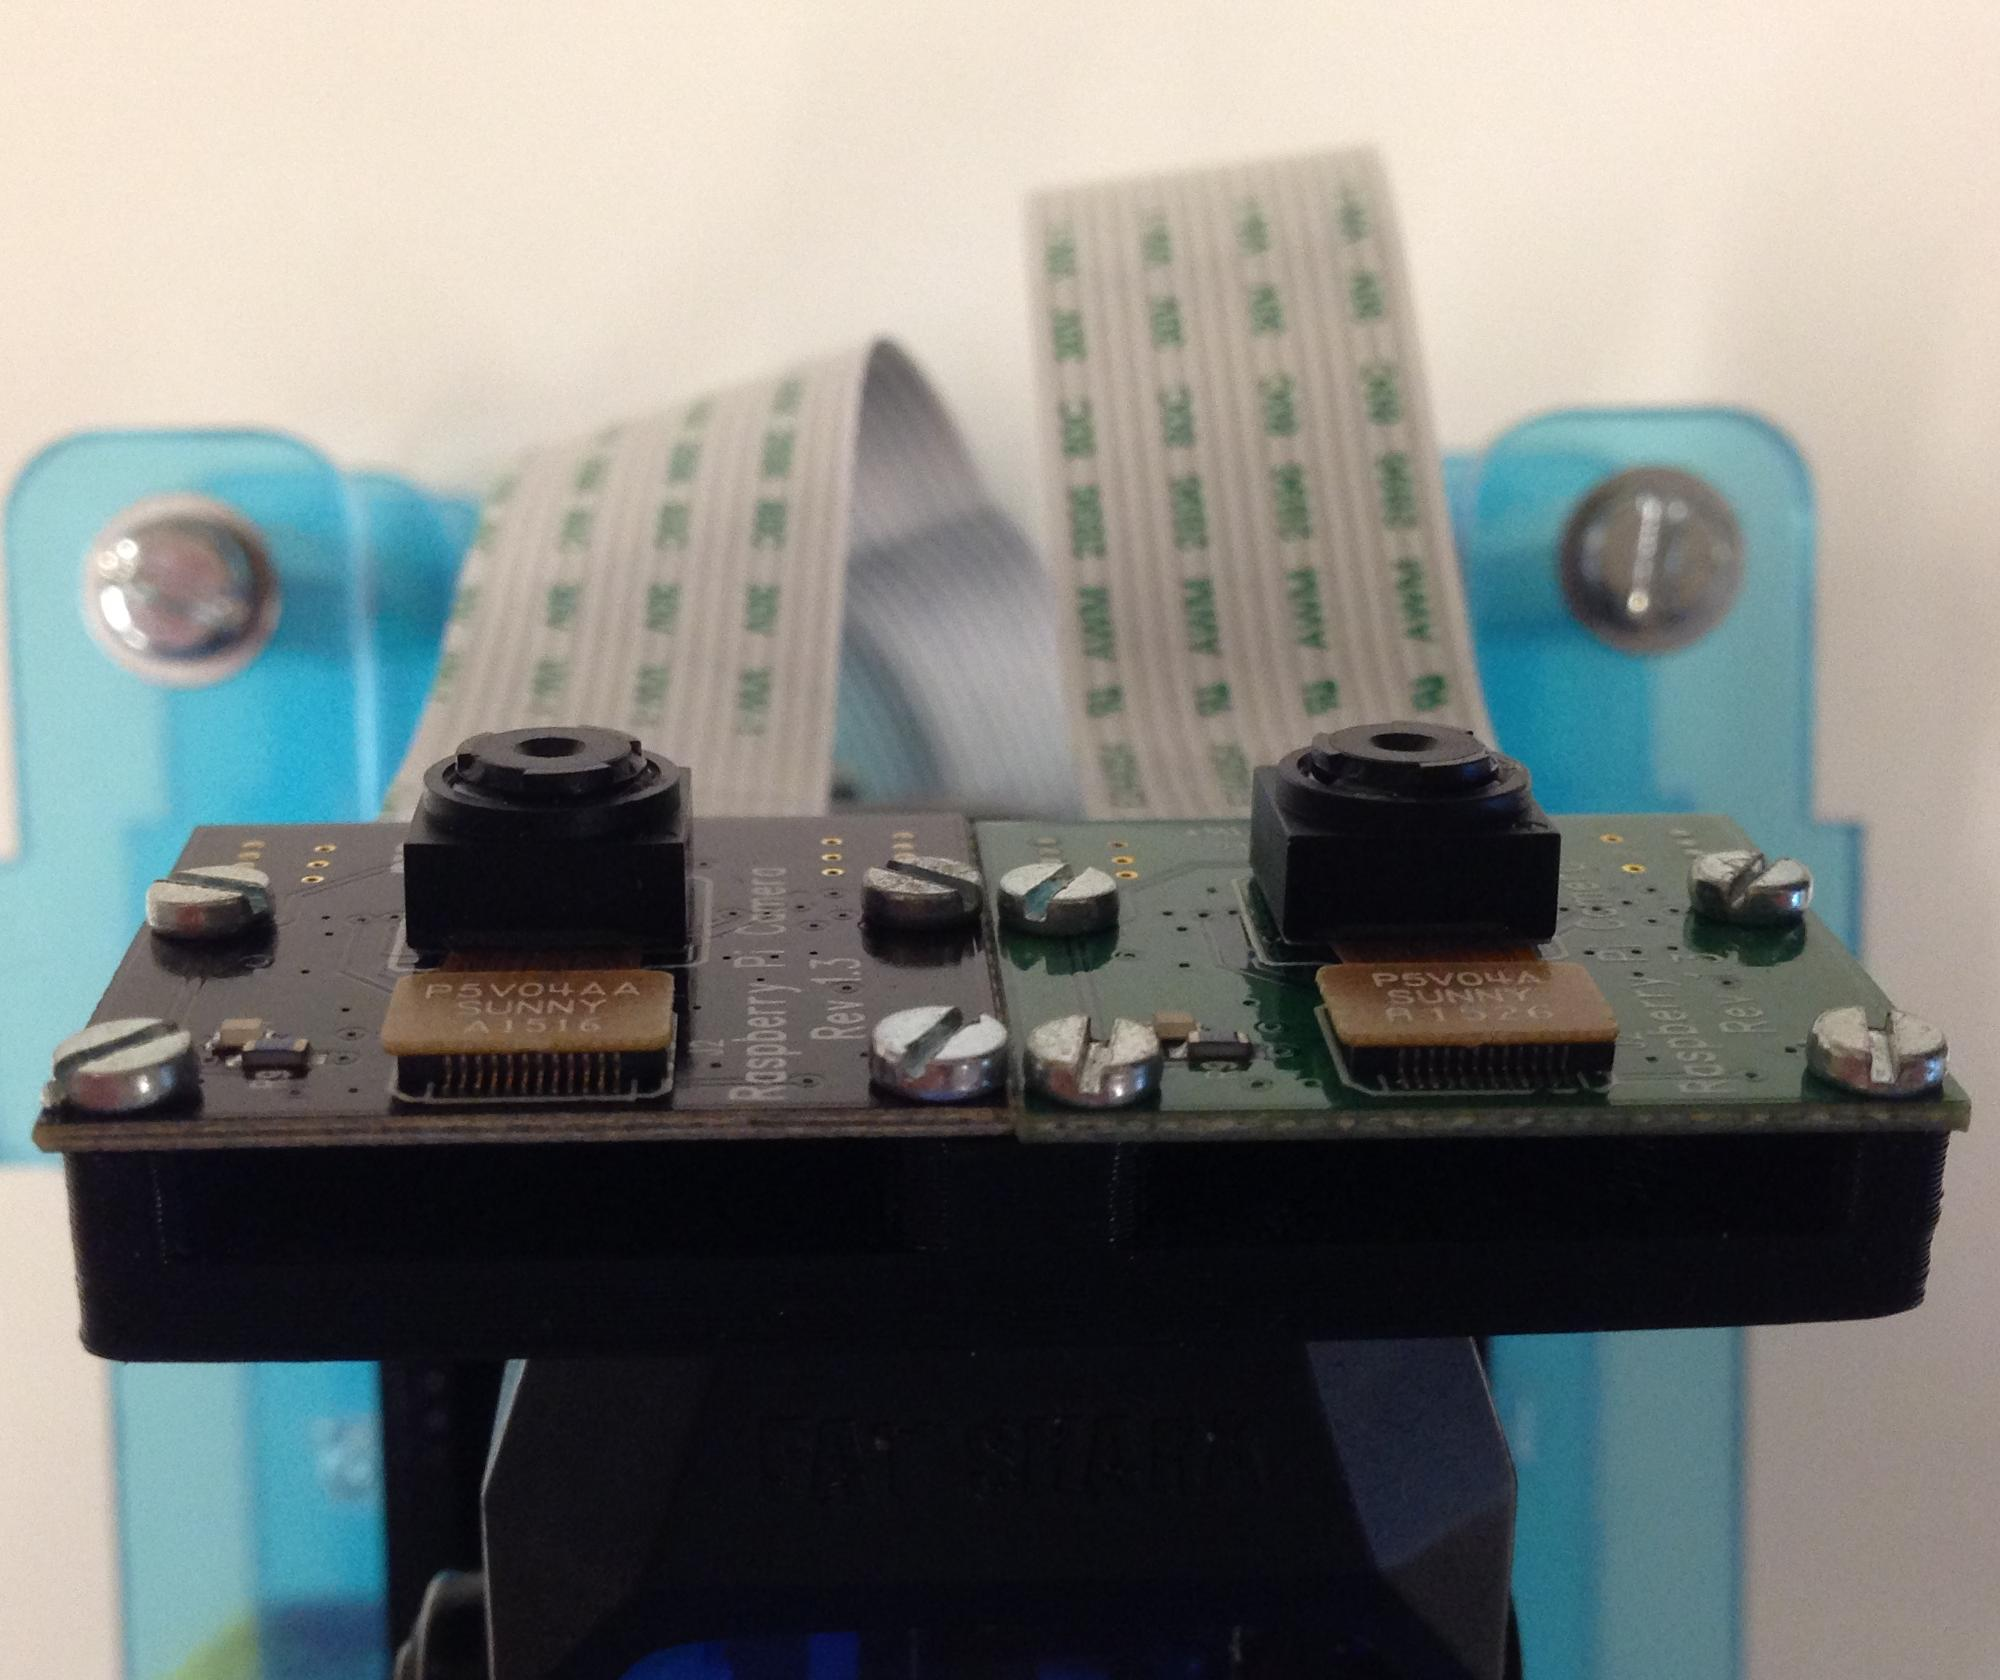
\includegraphics[width=\textwidth]{fig/dual_camera_no_filter_top_view.jpg}
                    \caption{Top view.}
                \end{minipage} \hspace{0.5em} %
                \begin{minipage}[b]{0.35\textwidth}
                    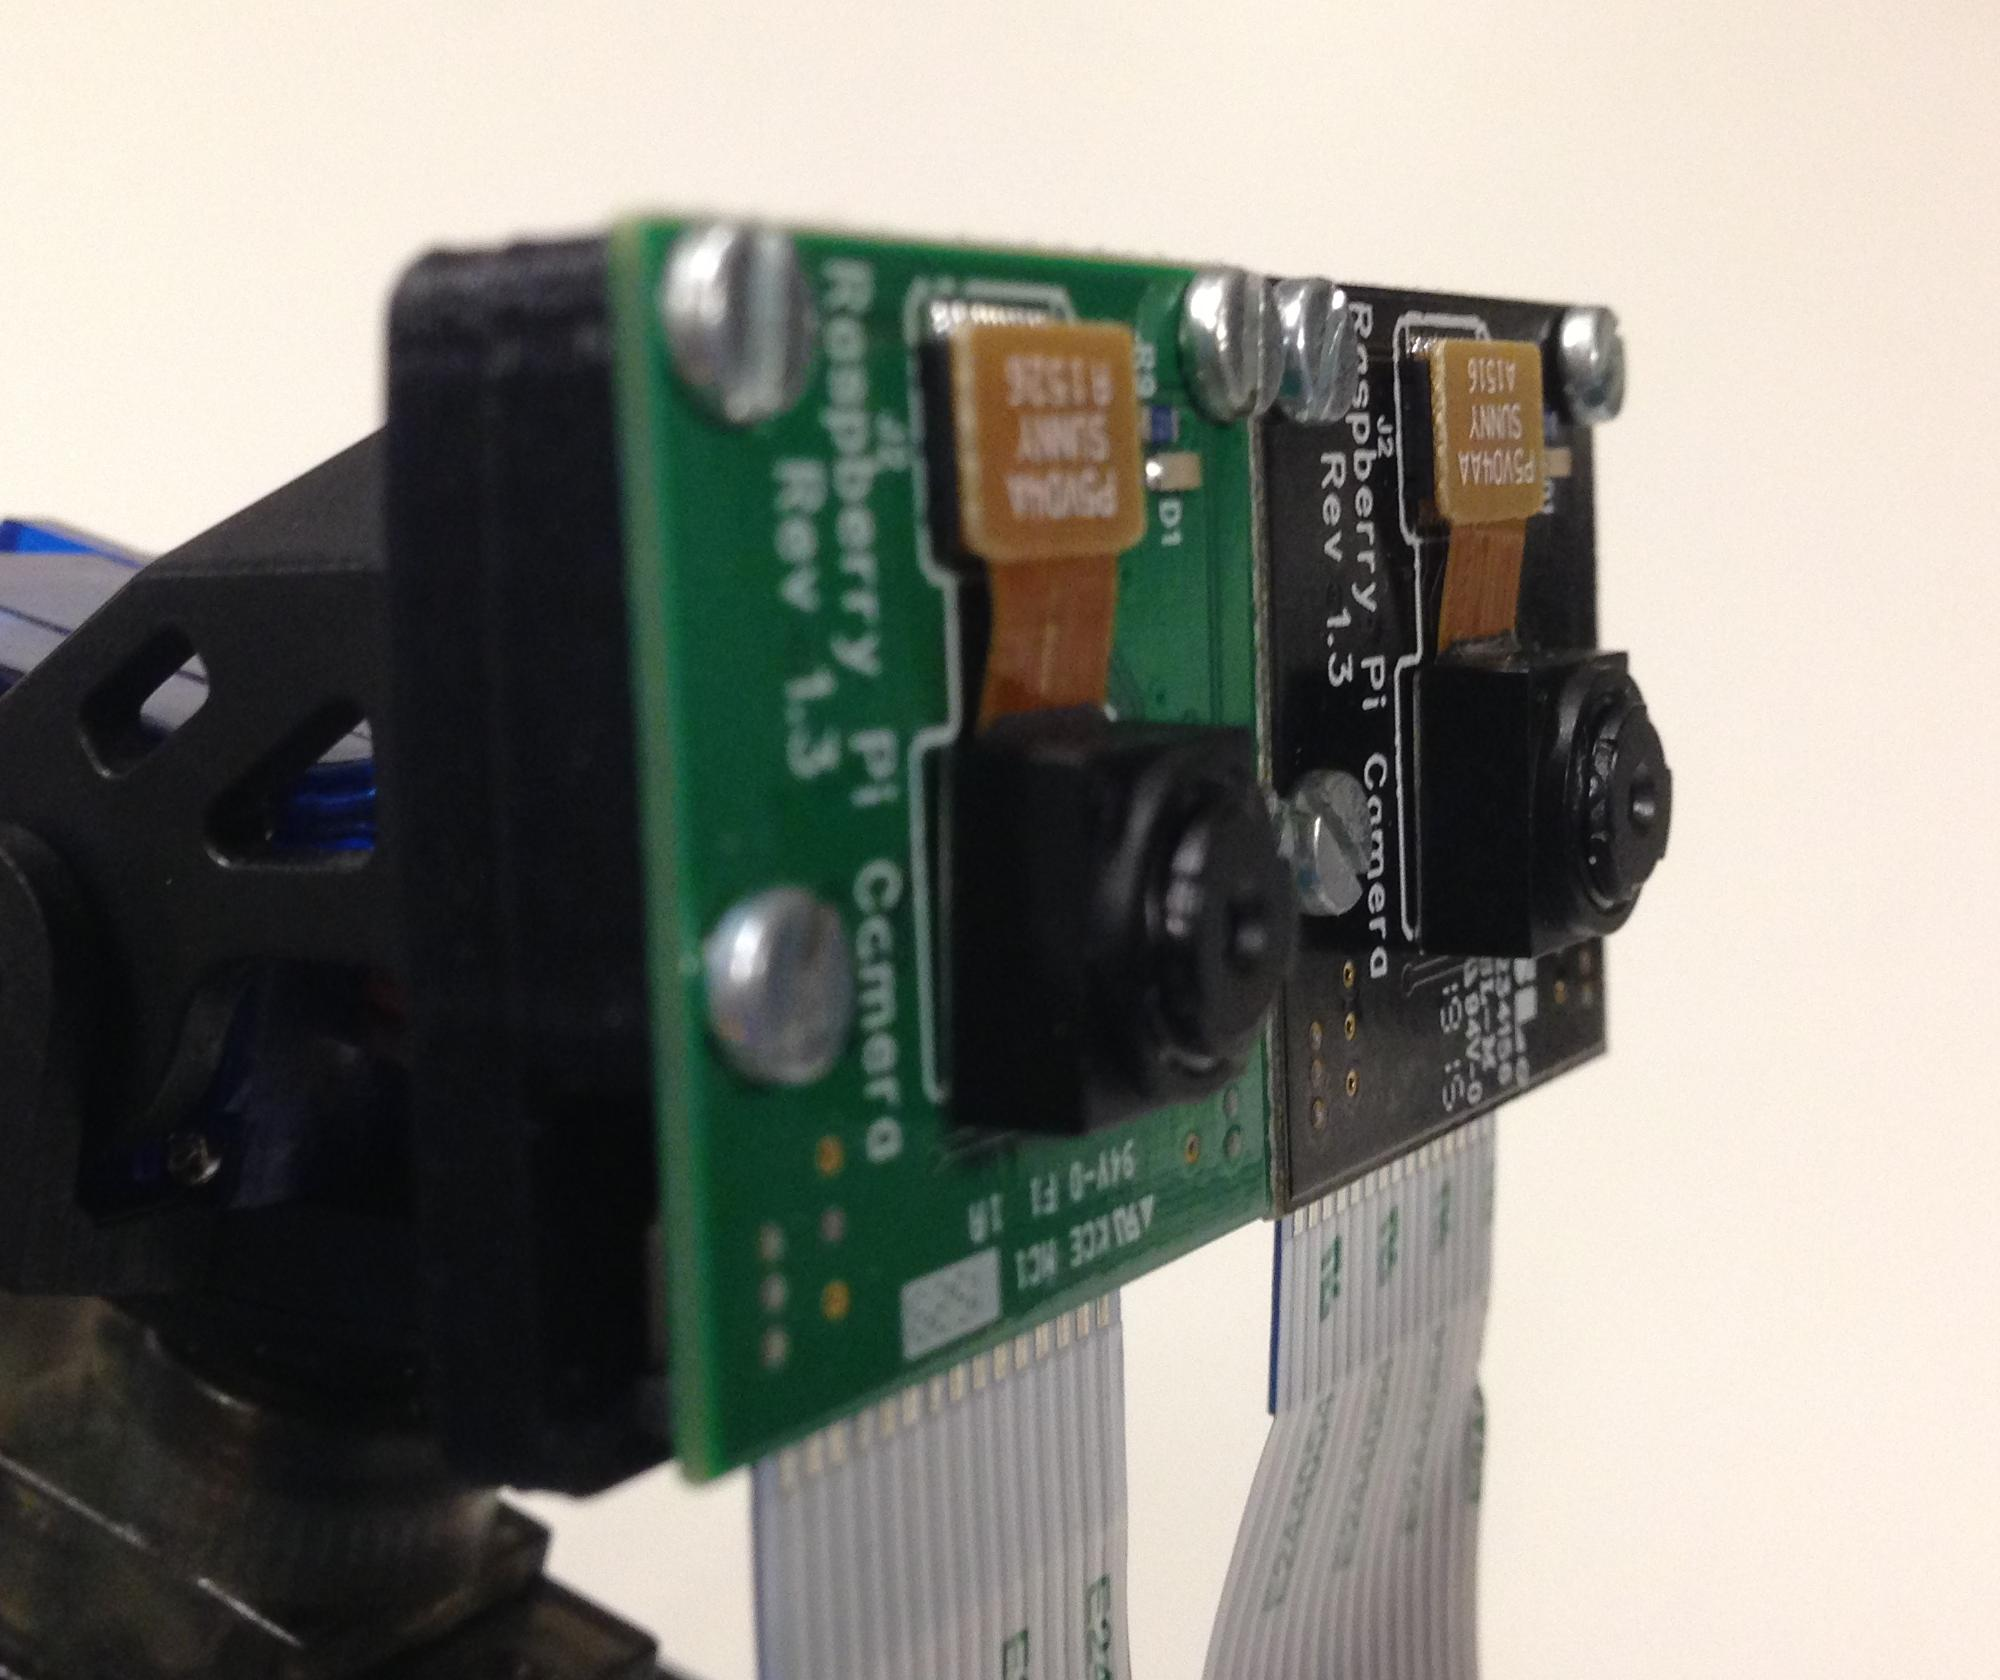
\includegraphics[width=\textwidth]{fig/dual_camera_no_filter_side_view.jpg}
                    \caption{Side view.}
                \end{minipage}
            \end{figure}

        \end{subsubsection}
    \end{subsection} % Hardware

    \begin{subsubsection}{Camera movement}
        To support pointing the camera in any direction, we needed a way to mechanically control the horizontal and vertical angle of the mount. This could be done by manually holding and orienting the 2 units, but results in unstable support. To get around this issue, we added a dedicated pan-tilt module.

        \medskip

        The pan-tilt module is composed of 2 servomotors (1 horizontal, and 1 vertical). A servomotor is a small engine that can rotate by 180 degrees subject to an input pulse of varying width. The figure below shows how a single servomotor responds to such a control pulse.

        \begin{figure}[!h]
            \centering
            \begin{minipage}[b]{0.3\textwidth}
                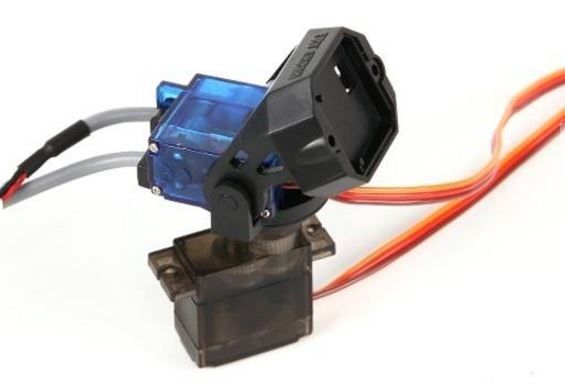
\includegraphics[width=\textwidth]{fig/pantilt_without_mount.jpg}
                \caption{Pan-tilt module.}
            \end{minipage} \hspace{0.5em} %
            \begin{minipage}[b]{0.5\textwidth}
                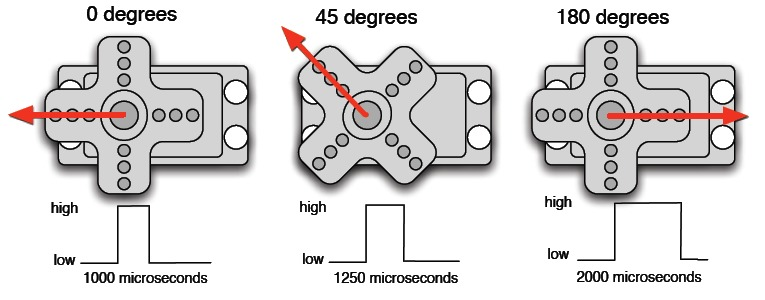
\includegraphics[width=\textwidth]{fig/servomotor_internals.jpg}
                \caption{Servomotor rotation under control pulse.}
                % http://sweb.cityu.edu.hk/sm2240/4/
            \end{minipage}
        \end{figure}

        To control the width of the input pulses for the two servomotors, we added a joystick to the system. One of the most commonly used joysticks on the market is the one that was available on the PlayStation~2 game console, so we went for the same model. Since the joystick has an {analog} interface, we needed to use an Analog-Digital Converter (ADC) to interface it with the RPi's GPIO pins. The RPi unfortunately doesn't have an internal ADC, so we added a very popular external one, the MCP3204.

        \medskip

        The ADC outputs 14-bit converted digital samples with a standard serial communication protocol (Serial Peripheral Interface, SPI). We use the CPU on the RPi to decode and save these converted samples.

        \medskip

        Once we have a digital reading of the values obtained from the joystick, we need to generate 2 control pulses for the pan-tilt module's servomotors. There are many ways to do this.

        \begin{enumerate}
            \item Use the CPU to explicitly create this control pulse: this unfortunately results in very high CPU utilization, as the pulse needs to be updated at a very high frequency.
            \item Use a dedicated hardware unit designed for generating PWM pulses. This provides the best performance as the CPU has almost nothing to do, but unfortunately the RPi only has 1 such unit, whereas we need 2 of them as we have 2 servomotors to control.
            \item Use a hybrid design where we employ a Direct Memory Access (DMA) unit to generate the control pulses. A DMA unit is a dedicated controller designed to efficiently copy data from one memory location to another. Since modern systems use \emph{memory-mapped} peripheral addressing, each peripheral is accessible at a certain address. This means that we can also use the DMA unit to write to a peripheral as if it were ``memory''. We programmed the DMA controller of the system to periodically write a modulated bit pulse to a GPIO port. This results in moderate CPU utilization, while being able to target any number of GPIO ports. We finally went for this solution.
        \end{enumerate}

        Figure~\ref{fig:servomotor_control_loop} shows the global hardware control loop used in our system.

        \begin{figure}[!h]
            \begin{center}
                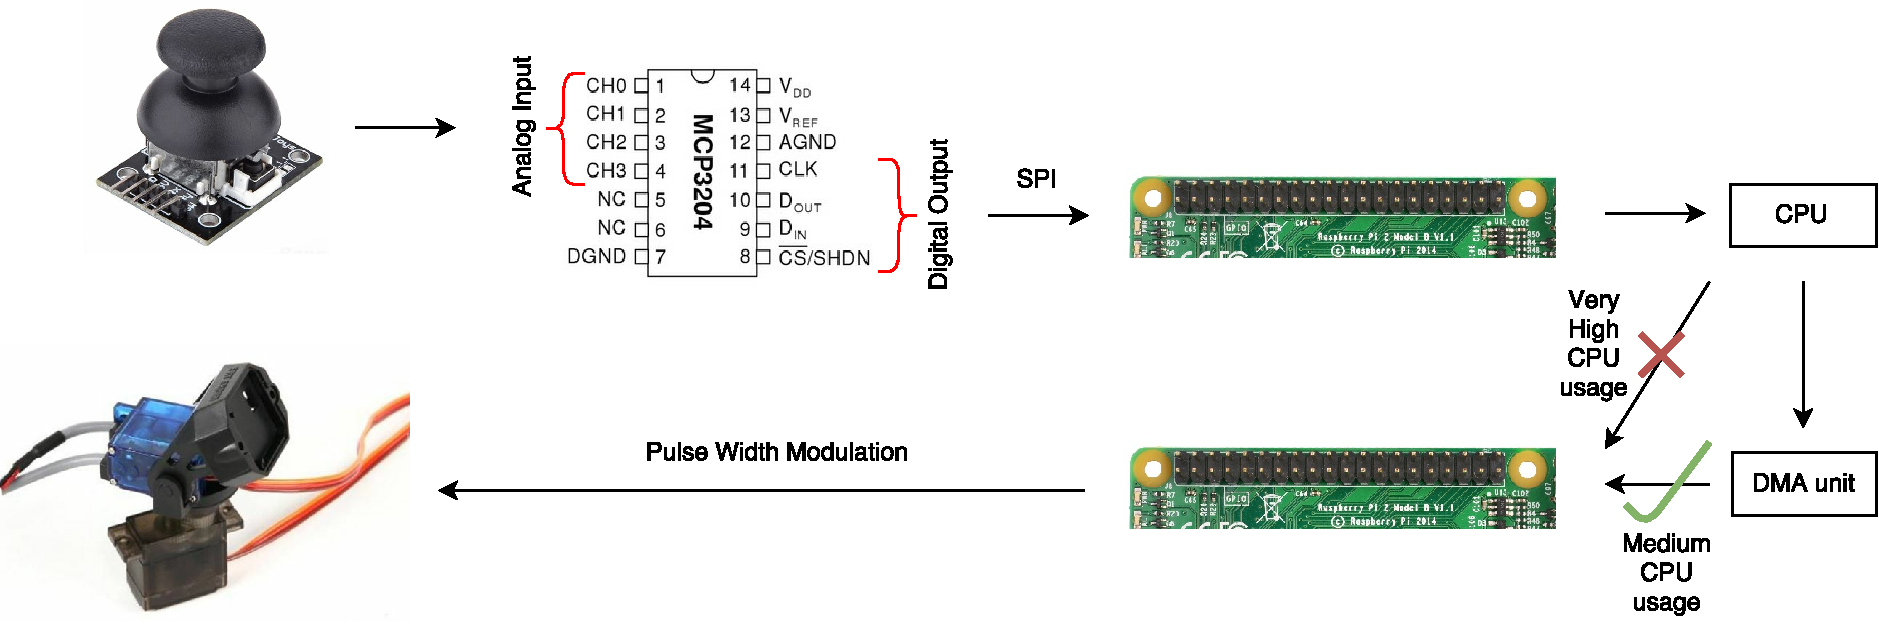
\includegraphics[width=\textwidth]{fig/rpi_wiring.pdf}
                \caption{Hardware control loop (simplified).}
                \label{fig:servomotor_control_loop}
            \end{center}
        \end{figure}
    \end{subsubsection}

    \begin{subsubsection}{Final hardware system}
        Finally, we put all components together in a stackable case and fixed all peripherals to it for easy transportation. Figure~\ref{fig:full_system} shows the full system once mounted.

        \medskip

        We need to obtain an RGB-only image, and an NIR-only image as the output of the acquisition system. The standard RGB camera comes with an NIR filter, so all is good on that front. However, the NoIR camera captures both visible and NIR light, instead of exclusively capturing NIR light

        \medskip

        To filter out the visible light, we use a small piece of exposed camera film. This camera film is fixed onto the NoIR camera with a (very sophisticated!) mounting system consisting of cello-tape.

        \begin{figure}[!h]
            \centering
            \begin{minipage}[b]{0.45\textwidth}
                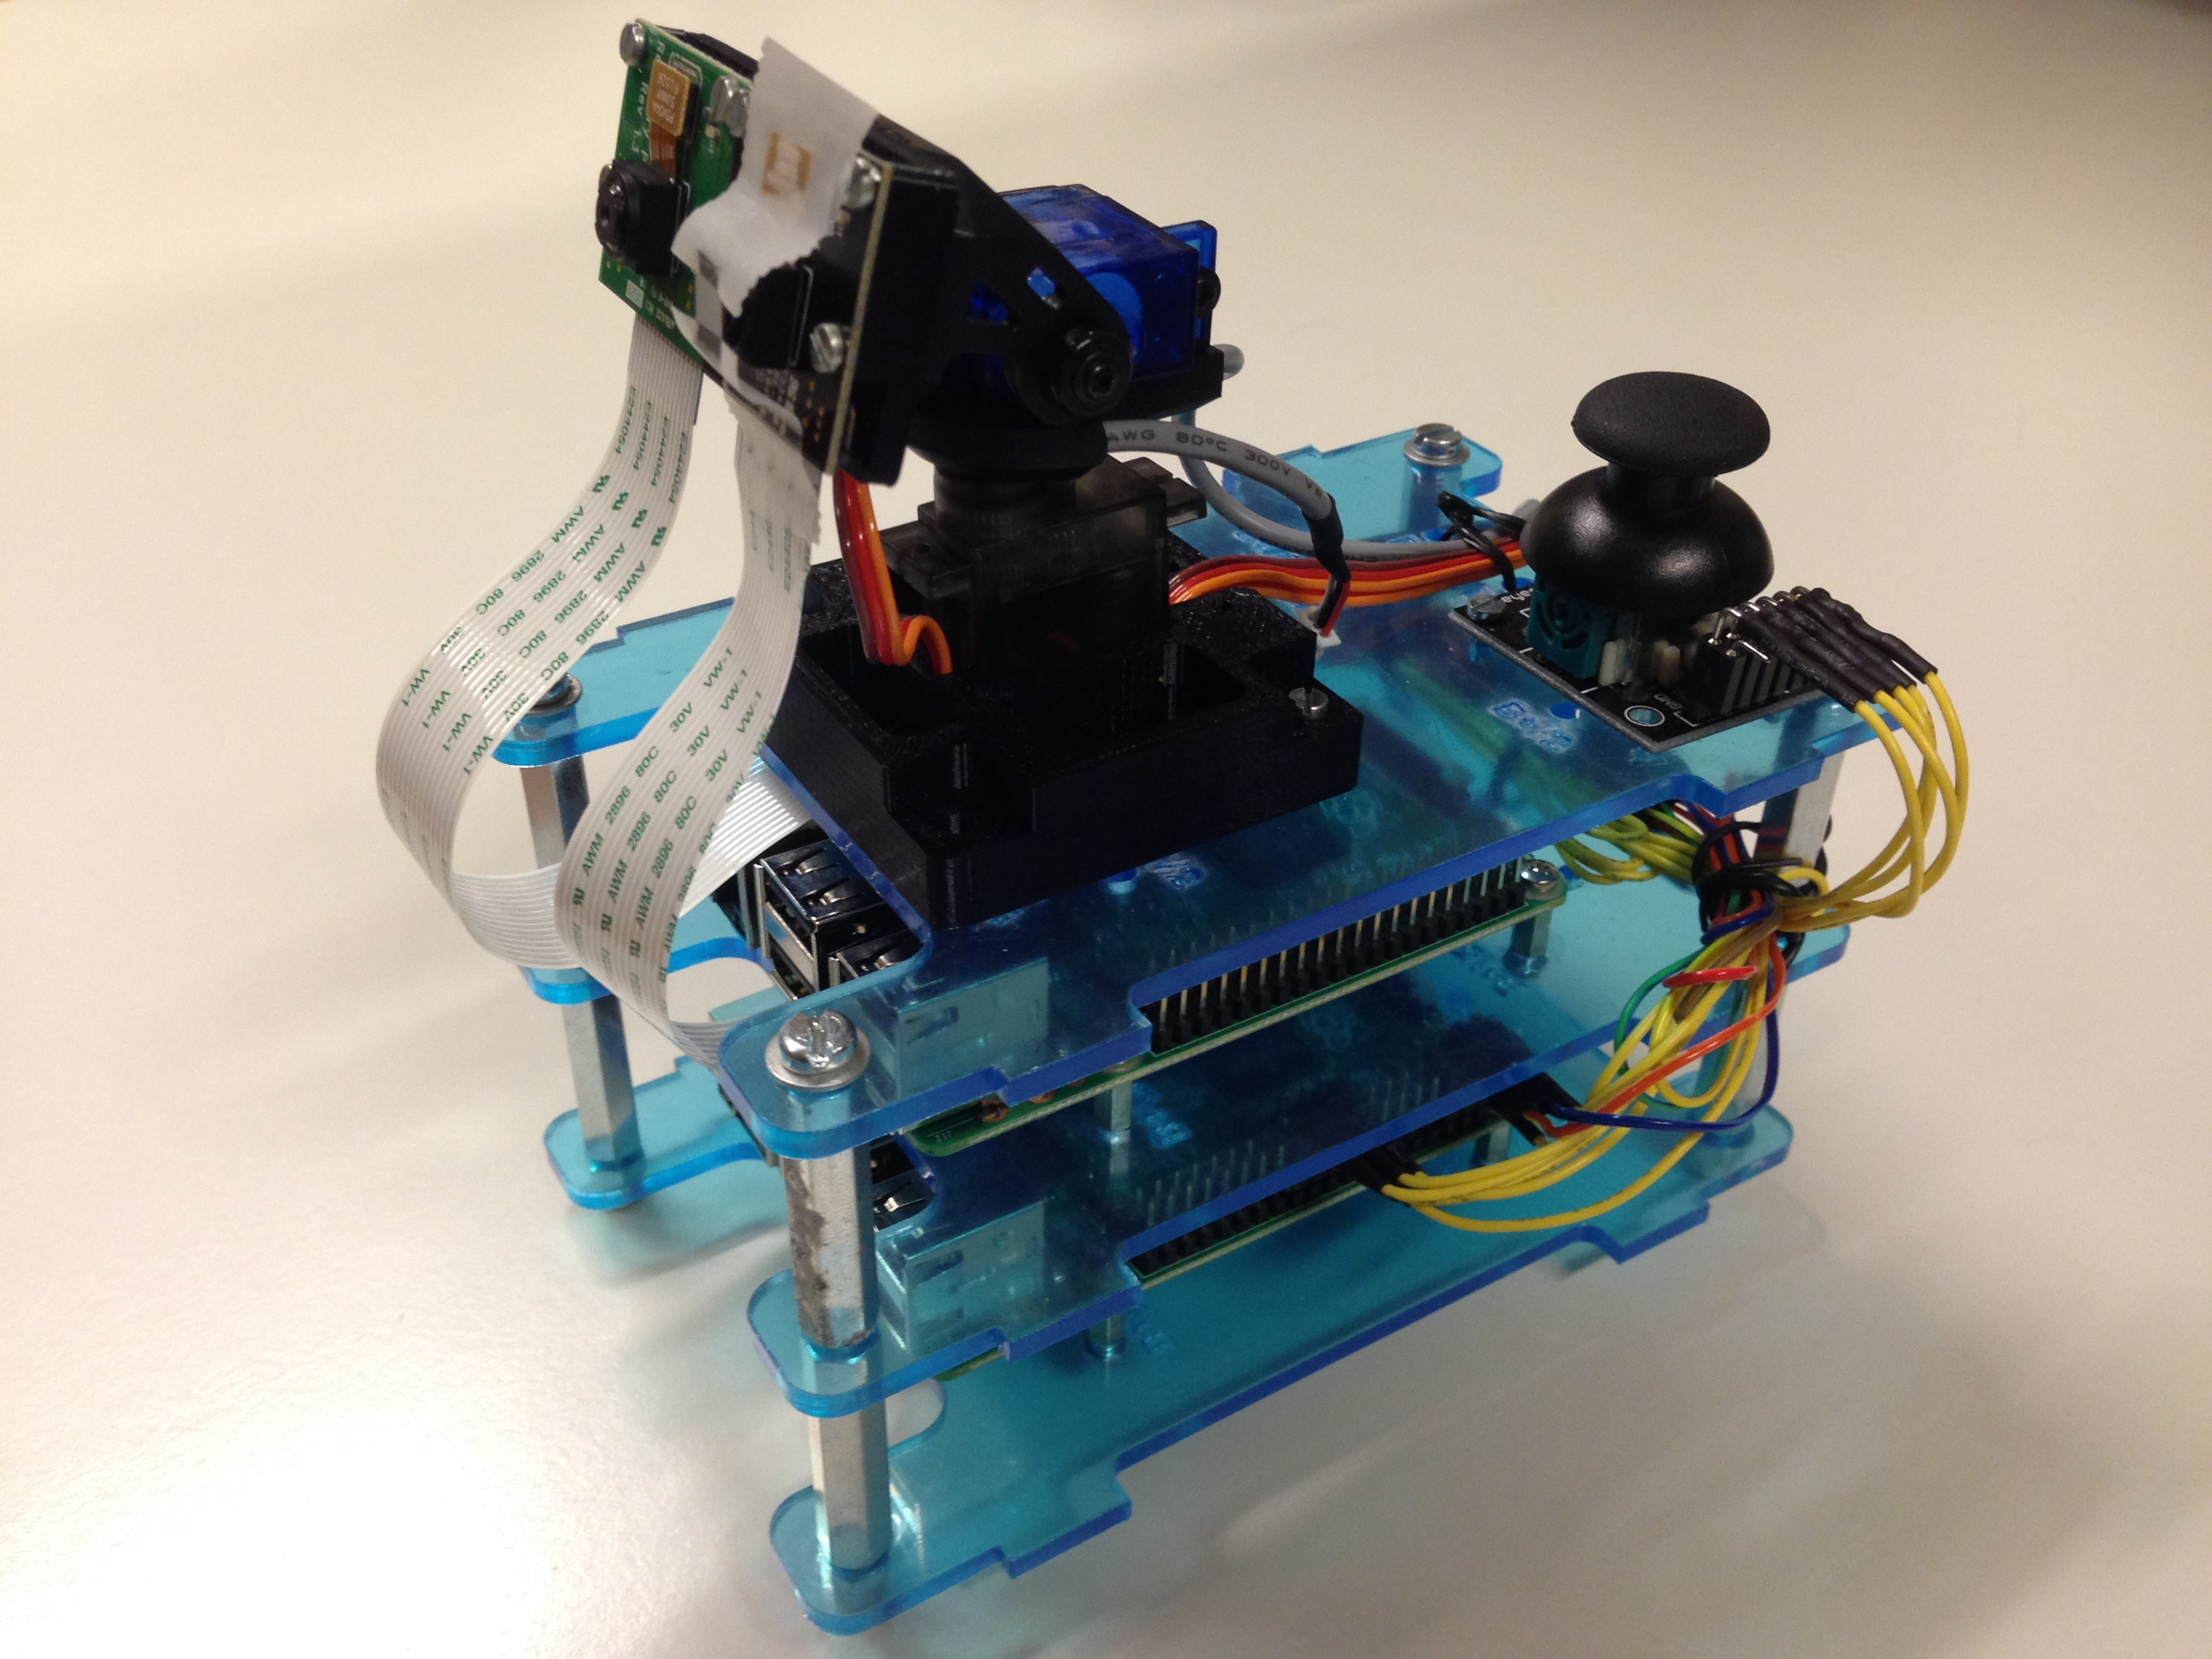
\includegraphics[width=\textwidth]{fig/full_system.jpg}
            \end{minipage} \hspace{0.5em} %
            \begin{minipage}[b]{0.45\textwidth}
                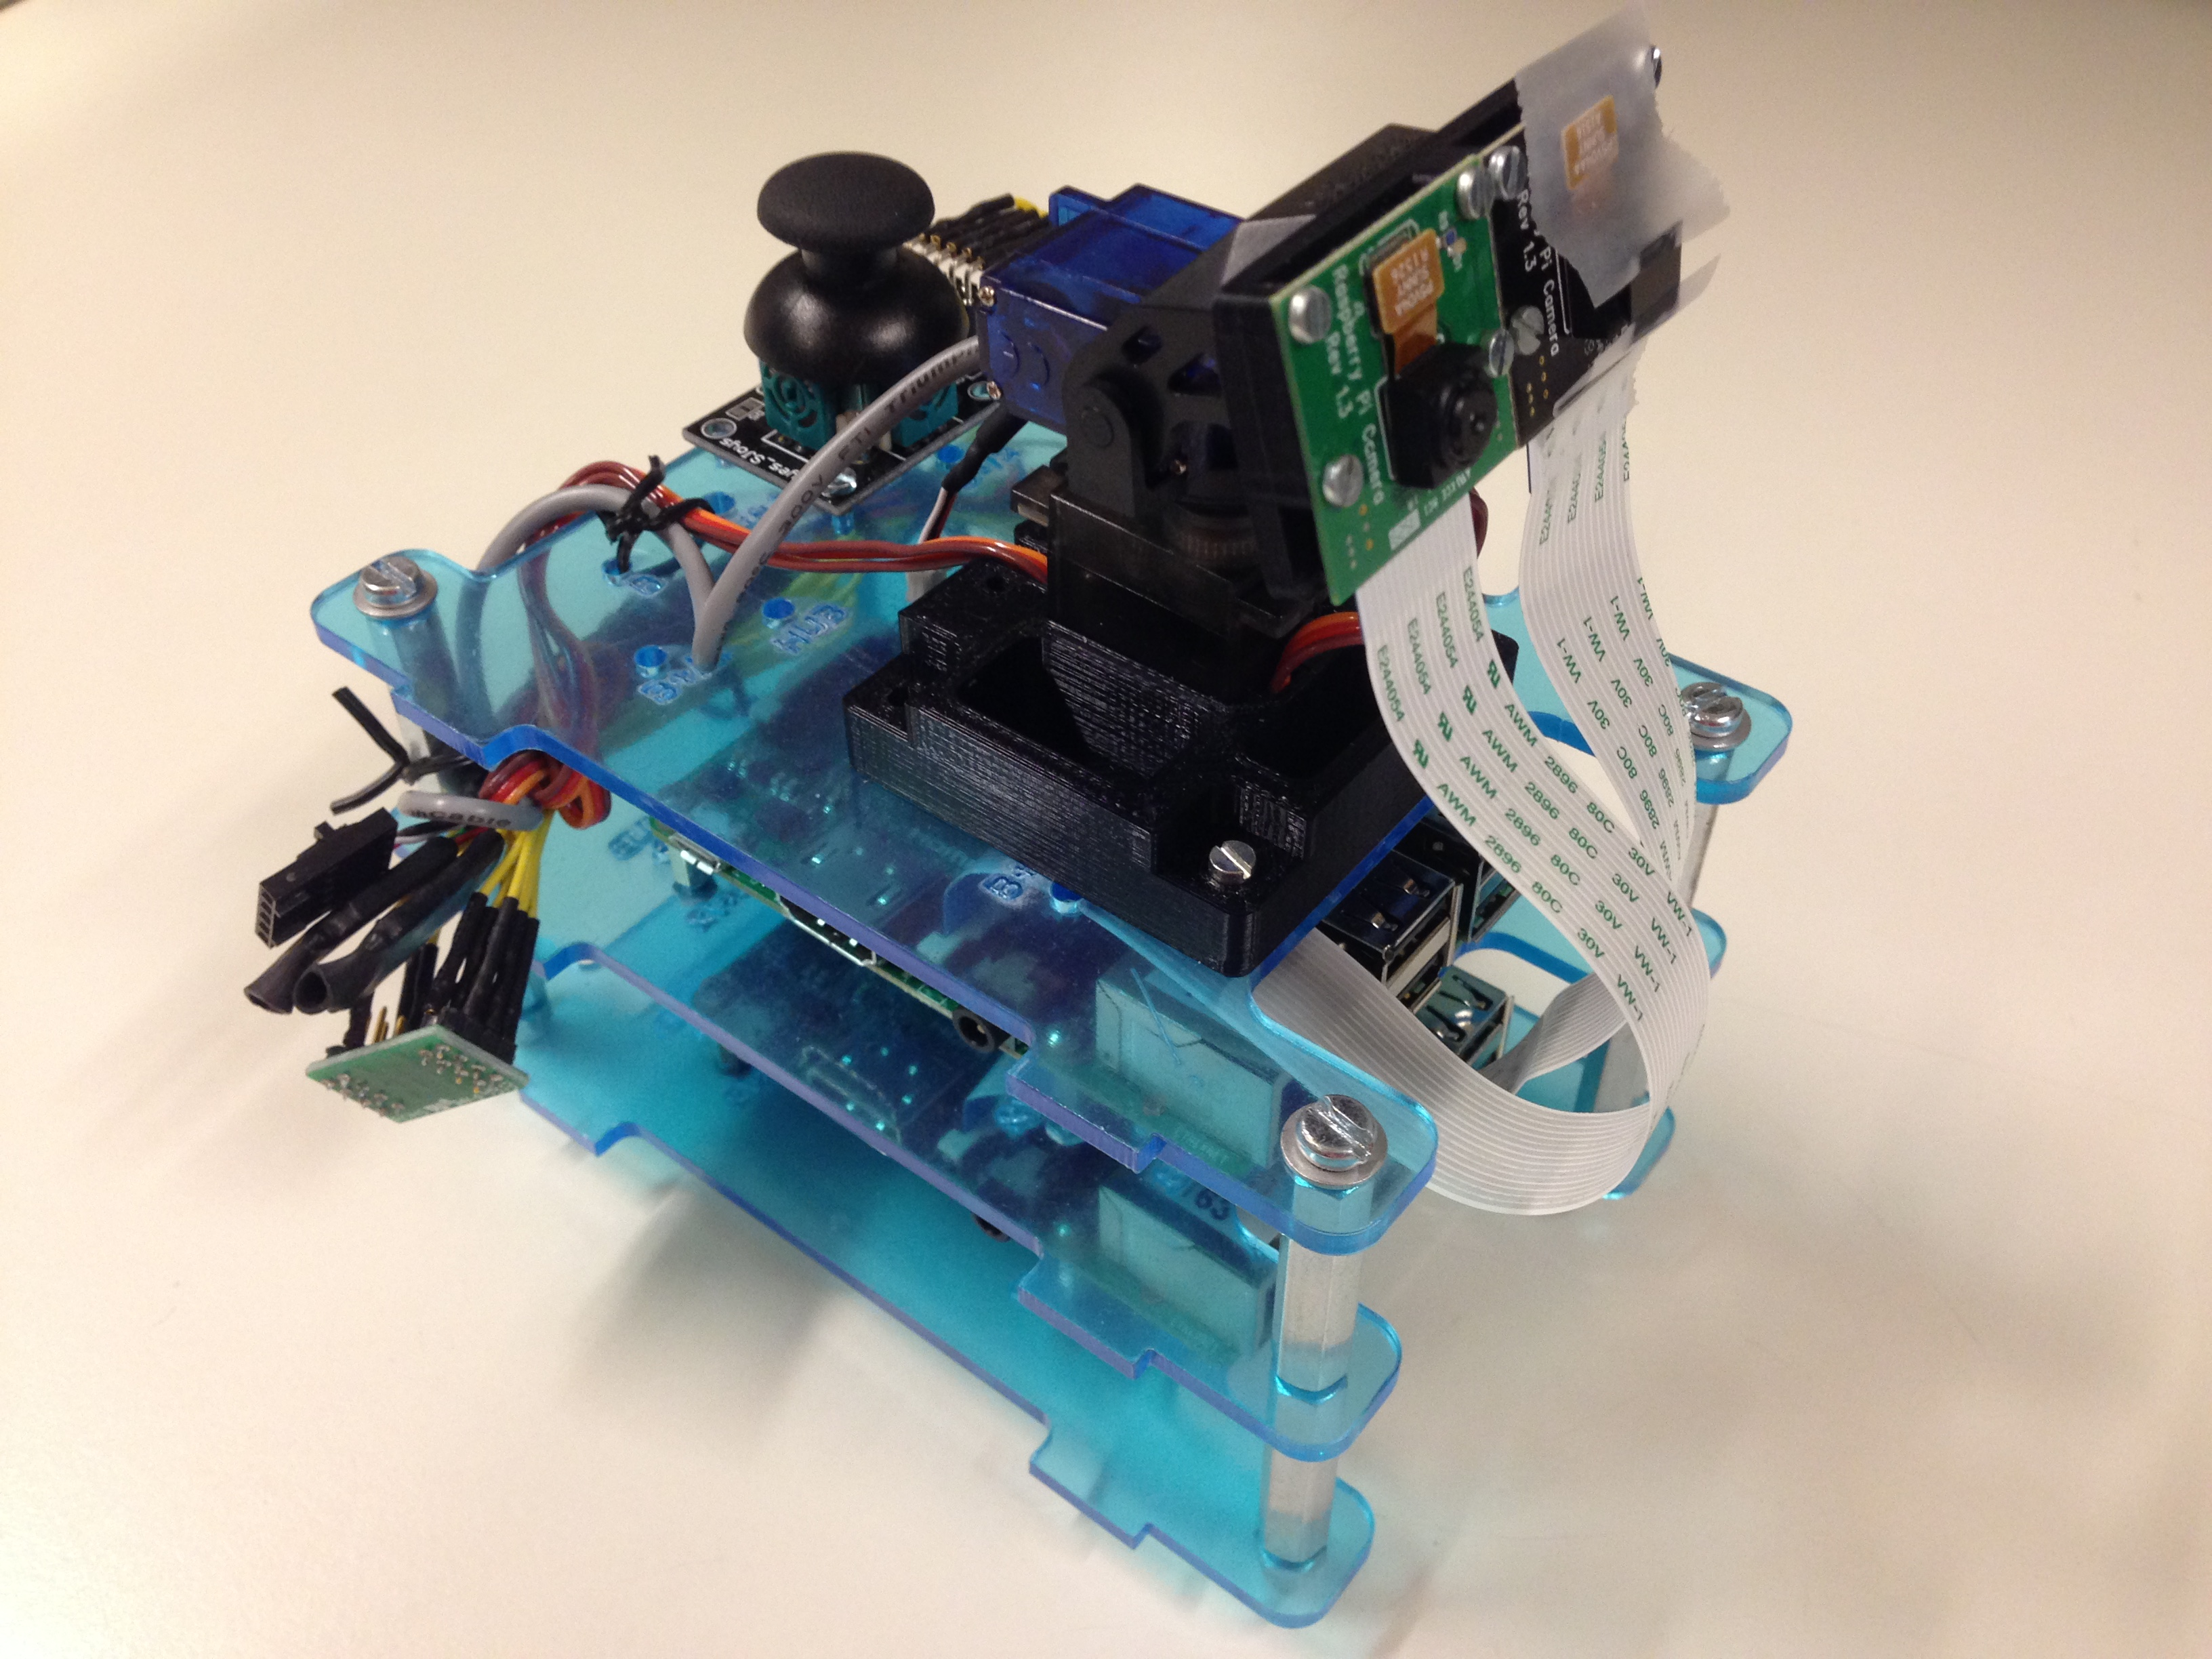
\includegraphics[width=\textwidth]{fig/full_system2.jpg}
            \end{minipage}
            \caption{Full acquisition system.}
            \label{fig:full_system}
        \end{figure}

    \end{subsubsection}

    \begin{subsection}{Synchronization}
        \label{sec:synchronization}
    \end{subsection} % Synchronization

    \begin{subsection}{Registration algorithm to align images}
        \label{sec:image_registration}
        \begin{subsubsection}{Theory}
            \textbf{Byte image:} image format where each pixel has a pixel value describing brightness. The values range between 0 and 255. Typically, zero is white and 255 is black.
            \\ \\
            \textbf{Keypoints:} something that stands out in the image and is consistent over several images. It is invariant towards certain transformations and insensitive to noise. Usually keypoints are found at corners and edges, due to the overlap between sections making it recognizable.
            \\ \\
            \textbf{Descriptors:} surrounding pixels of a keypoints. A keypoint with its descriptors creates an unique patch, working like a fingerprint for that part of the image.
            \\ \\
            \textbf{Kd-tree:} k-dimensional tree, data structure for organizing points in a k-dimensional space.
            \\ \\
            \textbf{Homography:} a reweighted version of the least squares method (measuring the smallest error to a motion parameter). The difference between least square method and homography is subtle but homography works better on non-linear relationships.
            \\ \\
            \textbf{RANSAC:} RANdom SAmple Consensus, a method to remove outliers in the matching process. An outlier is a match which is incorrect.
        \end{subsubsection}

        \begin{subsubsection}{Alignment of images}

            In the registration part of the project, the main purpose is to align the two images so they later can be merged. To do this, a motion parameter needs to be found that can move one image to suit the other. For this purpose, the OpenCV library has been imported. Below is a description of the steps taken in the registration process.

            \begin{itemize}
                \item Open up the images and convert their format to byte images, regardless of previous format. This is saved into an array, where each element is a list with all values for the pixels of the first row of the image.

                \item Locate keypoints and descriptors using the SIFT-algorithm. SIFT has the size of 16 x 16 windows around the keypoint. It computes the gradient for each pixel, which is important in the preprocess for matching.

                \item Extract the keypoints and descriptors, through a detector, extractor and compute functions.

                \item Match the patches of keypoints and descriptors over the images.The Flann Index Tree and a ratio test is performed. The Flann Index is a fast way of approximating the nearest neighbor to a point in a large data set and for high dimensional features.The constructed index is a randomized kd-tree which is searched through in parallel, in our case in five trees. It computes the distances between pairs of features. The ration test put a threshold of the matches, only choosing the closest 70 \% in distance.

                \item When appropriate matches are found, it’s time to get the motion parameter with the best accuracy in regard to translation and rotation. Homography and RANSAC is used, since the relationships between the motions are nonlinear. Homography evaluate the parameters in regard to how big errors they provide, choosing the best motion parameter. RANSAC is a method to remove outliers.

                \item Warp the source image to the destination image, meaning make the transformation.

                \item Open up the source image, the destination image and the warped source image. An image has been created consisting only of the shared content of the two input images, making it appear to be taken from the same perspective as one of the input images and with the possible to merge them.

            \end{itemize}
        \end{subsubsection} % Registration algorithm

    \end{subsection} % Method
\end{section}

\begin{section}{Applications}

    \begin{subsection}{Skin Smoothing}
        \label{sec:skin_smoothing}
    \end{subsection}


        \begin{subsection}{Shadow Detection}
            \label{sec:shadow_detection}
            Another feature that we implemented in our project is a shadow detection algorithm. From one pair of registered RGB and NIR images, this part aims to automatically detect shadows in a fast way by using the properties of the near-infrared information. The idea behind is that dark objects that are often detected as shadows in traditional RGB shadow detection algorithms have a much higher reflectance in the NIR spectrum. This method is build around three main observations: The first one is that shadows are generally darker than their surroundings. Second, a considerable number of dark objects in the visible spectrum are brighter in the NIR one. The last one is that most illuminants have a specific behavior in the NIR.
            \\ \\
            Our algorithm follows the one described in the paper [0000]. It takes as input the pair of registered RGB and NIR images computed in \ref{sec:image_registration} and output a binary mask revealing the pixels estimated as under shadow. Its operation is briefly explained in the following paragraphs. We can easily divide it in three parts: Shadow candidates, Color to NIR Ratios and Binary Shadow Mask.
            \\ \\


            \begin{subsubsection}{Shadow Candidates}
                \label{sec:shadow_candidates}
                The first task is to find the areas where the probability of finding a shadow at this place is high. We call this the shadow candidate map. Because darkness in both visible and NIR images is a condition of shadow presence, we need to compute a shadow candidate map for both. For the visible one we compute the brightness of the image to whom we apply a non-linear mapping on it to obtain a better result. The NIR one is pretty straightforward because we only need to apply the non-linear mapping on the near-infrared image. The final shadow candidate map is simply the multiplication of the two to take in account the two conditions.
            \end{subsubsection}

            \begin{subsubsection}{Color to NIR Ratios}
                \label{sec:color2NIR_ratios}
                The shadow candidate map is already giving a good intuition about shadow presence but it is possible to upgrade it with the help of color to NIR ratios. The key insight here is that the difference between the visible and NIR bands for many shadow creating illuminants is distinctive. For example, the illuminant spectral power of the skylight is greater for the visible light than for the NIR while their are close to equal under sunlight. we can exploit this difference and compute the ratio image between the RGB and the NIR image. This ratio will be greater than one for skylit regions and around one for sunlit regions. Let's not forget to take the maximum ratio over the three color channels to obtain the better results. We also have to handle the case where the ratio could tends to infinity when the pixel intensity of the NIR image tends to zero. The shadow map found in \ref{sec:shadow_candidates} contains all possible shadows but can also include dark objects. By combining this with the ratio image, we obtain a pretty nice shadow detector .
            \end{subsubsection}

            \begin{subsubsection}{Binary Shadow Mask}
                \label{sec:binary_shadow_mask}
                In the last step, we combine the results of \ref{sec:shadow_candidates} and \ref{sec:color2NIR_ratios} by multiplying the complementary of both. This give us a nice continuous shadow map. Finally, we want to threshold this shadow map to distinguish shadow from non-shadow area as a binary shadow mask. The key to find a good threshold value is to compute the histogram of the image and then set the threshold value to the first valley of the histogram. The first valley is defined as the smallest valued bin of the histogram where the two neighboring bins on both sides have larger, increasing values. The resulting binary image indicates which pixels are shadow and which aren't.

            \end{subsubsection}

        \end{subsection}

\end{section}

\begin{section}{Conclusion}
    \label{sec:conclusion}
\end{section}

% \begin{thebibliography}{9}

%     \bibitem{lamport94}
%     C. Fredembach, N. Barbuscia and S. Süsstrunk,
%     \emph{A device and an algorithm for the separation of visible and near infrared signals in a monolithic Silicon sensor},
%     Addison Wesley, Massachusetts,
%     2nd edition,
%     1994.

% \end{thebibliography}

\begin{section}{Credits}
    \begin{description}
        \item [Dajana Vlajic \& Rebecka R{\H o}nnb{\"a}ck] Image registration
        \item [Florian Zimmermann] Raspberry Pi operating system setup \& Synchronization
        \item [Josselin Vallee] Skin smoothing
        \item [Sahand Kashani] Dual-camera mount, Joystick \& Dual-servomotor control
        \item [Yann Perret] Shadow detection
    \end{description}
\end{section}

\end{document}
